\documentclass[12pt]{article}

  \usepackage[polish]{babel}
  \usepackage[utf8]{inputenc}
  \usepackage[T1]{fontenc} 
  \usepackage{hyperref}
  
  \usepackage[numbers,sort&compress]{natbib}
  \usepackage{hypernat}

  \usepackage{graphicx}
  \usepackage{epstopdf}

  \usepackage[footnotesize,bf]{caption}

  \usepackage{amsmath}
  \usepackage{latexsym}

  \usepackage{titlesec}
  \titlelabel{\thetitle.\quad}

  %strona tytulowa
  \usepackage{strona_tytulowa}


  \title{Badanie dynamiki złożonych sieci neuronów o potencjale ciągłym
  z szumem synaptycznym i opóźnieniami w transmisji potencjałów}
  \author{Tomasz Stachewicz}

  %polecenia zdefiniowane w pakiecie strona_tytulowa.sty
  \uczelnia{Politechnika Warszawska}
  \instytut{Wydział Fizyki, Zakład Układów Złożonych}
  \promotor{dr. hab. Andrzeja Krawieckiego}
  \praca{PRACA DYPLOMOWA}
  \rok{2011}
  \draft  %odkomentowac jesli wydruk ma byc draftem -- bedzie informacja na stronie tytulowej
  %koniec polecen zdefiniowanych przez pakiet strona_tytulowa.sty



\begin{document}

  \thispagestyle{empty}               %na tej stronie: brak numeru
  \stronatytulowa                     %strona tytulowa tworzona przez pakiet strona_tytulowa.tex

  \tableofcontents
  \newpage

  \section{Wstęp}

Przedmiotem niniejszej pracy jest badanie rezonansu stochastycznego w matematycznych modelach układach neuronów biologicznych, trakowanych jako układy z pamięcią i połączonych w sieci przestrzennie rozciągłe.

Rezonans stochastyczny jest zjawiskiem polegającym na wzmocnieniu przez układ słabego, zewnętrznego sygnału periodycznego w obecności szumu w taki sposób, że sygnał wynikowy (zachowanie układu) także jest periodyczny i o częstotliwości takiej jak częstotliwość owego zewnętrznego sygnału. Rezonans Stochastyczny obserwuje się w m.in. elementach progowych oraz wzbudnych (excitable). Matematyczne modele neuronów biologicznych wraz z rezonansem stochastycznym i układami z pamięcią stanowią trójkę gałęzi matematyki i fizyki, które składają się na przedmiot niniejszej pracy.

Ze względu na złożoną postać matematyczną, rozpatrywanie tego rodzaju zagadnień metodami analitycznymi jest trudne (w skrajnych przypadkach niemożliwe). Z tego powodu podstawą niniejszej pracy jest autorskie oprogramowanie napisane do symulacji badanych układów.

Pierwszym etapem pracy było zbadanie modelu pojedynczego neuronu biologicznego (element wzbudny), w którym w pewnym zakresie parametrów obserwuje się zjawisko rezonansu stochastycznego. Następnie z takich neuronów budowano jednowymiarowe macierze (łańcuchy) elementów oddziałujących ze sobą poprzez przekazywanie potencjałów czynnościowych.

W zależności od sposobu budowy takich układów zaobserwowano różne zjawiska. Najważniejsze z nich to wzmacnianie (kontrola) rezonansu stochastycznego w układach bez opoźnień i odbierających sygnał periodyczny w tej samej fazie oraz uzyskanie takiego samego wzmocnienia w układach odbierających sygnał periodyczny w różnej fazie (wpływ rozciągłości przestrzennej), ale z opóźnieniami w transmisji potencjałów kompensującymi różnice faz.
  \newpage

    \section{Podstawy Teoretyczne}
  
  \subsection{Rezonans Stochastyczny}
  
  Rezonans stochastyczny (SR) jest zjawiskiem występującym (między innymi, na potrzeby niniejszej pracy) w układach pobudzanych co najmniej dwoma sygnałami, z których jeden jest periodyczny, drugi natomiast jest szumem. O występowaniu rezonansu stochastycznego mówimy, kiedy nałożenie sygnału periodycznego i niezerowego szumu na wejściu układu skutkuje wysoką periodycznością sygnału wyjściowego.
  
  Powyższe oznacza, że odpowiednio dobrany szum potrafi wzmacniać i wydobywać z układu sygnał periodyczny. Szum, zazwyczaj traktowany jako zjawisko niepożądane ze względu na obniżanie dokładności pomiaru, w układach z rezonansem stochastycznym staje się zjawiskiem jak najbardziej pożądanym. 
  
  Podstawową wielkością używaną przy badaniu rezonansu stochastyznego jest stosunek sygnału do szumu (signal-to-noise ratio, zwany dalej SNR), określający skuteczność wzmocnienia składowej periodycznej w wyniku działania szumu.

  Istnieje wiele układów z rezonansem stochastycznym, od podwójnej studni potencjału, przez układy progowe po układy równań różniczkowych.

  \subsubsection{Układ Bistabilny}
  \label{sec:uklad_bistabilny}

  Najprostszym w rozpatrywaniu analitycznym rezonatorem stochastycznym jest cząstka poruszająca się w  podwójnej studni potencjału, opisywanej równaniem

  \begin{equation} \label{sr:1}
    V_t(x) = \frac{1}{4} x^4 - \frac{1}{2} x^2 + \lambda_0 cos(2 \pi \epsilon t) x
  \end{equation}

  gdzie t jest czasem (modulacja potencjału w czasie), a $\lambda_0 > 0$ stałą dobraną tak, że potencjał $V_t(x)$ ma zawsze dwa lokalne minima. Taki model nazywa się asymetrycznym potencjałem podwójnej studni i zmienia się on w sposób ciągły w czasie z okresem $\frac{1}{\epsilon}$.

  Sygnał periodyczny moduluje względną wysokość obu studni poencjału tak, że przez pierwszą połowę okresu głębsza jest ''prawa'' ($x>0$), a przez drugą połowę okresu -- ''lewa'' ($x<0$) studnia potencjału.

  Jeśli zobrazować sygnał wejściowy jako podnoszący minima potencjału, to schematycznie można przedstawić taki układ następująco:

  \begin{figure}
    \includegraphics[width=80mm]{images/sr.jpg}
    \caption{obrazowe przedstawienie rezonansu stochastycznego w podwójnej studni potencjału}
  \end{figure}


  Ze względu na prostą postać analityczną, zależność SNR od szumu jest także znajdowalna w sposób analityczny:

  Wykreślone na podstawie powyższego wzoru wykresy SNR odpowiadają danym zebranym w symulacjach i przedstawiają się następująco:



  \subsubsection{Układ Progowy}
  \label{sec:uklad_progowy}

  W zastosowaniach praktycznych (wzmacnianie sygnałów) oraz symulacjach popularny jest rezonator monostabilny, progowy (układ niedynamiczny). Mechanizm jego działania polega na wysłaniu przez układ ''szpilki'' potencjału kiedy suma wymuszenia periodycznego i szumu przekroczy (wznosząco) wartość progową. Taki rezonator był badany doświadczalnie (symulacje, realizacja elektroniczna) i teoretycznie w pracy \cite{gingl_kiss_moss}. Dokładniejsza dyskusja teoretyczna rezonatora progowego była przedmiotem prac \cite{blondeau_e53} i \cite{blondeau_e55}. Widmo mocy takiego układu posiada wysokie i wąskie piki dla częstotliwości wejściowego sygnału i jej wielokrotności, stąd też jest bardzo wdzięcznym obiektem badań nad rezonansem stochastycznym.

  Sygnał wejściowy w układzie badanym przez Gingla \cite{gingl_kiss_moss} jest po prostu sumą sygnału periodycznego i szumu:

  \begin{equation} \label{sr:gingl}
    v_{in}(t) = A sin (\omega_0 t) + D \xi(t)
  \end{equation}
  
  Wyniki uzyskane przez Gingla przedstawia grafika \ref{fig:graphics:gingl}. 

  \begin{figure}
    \includegraphics[scale=0.8]{images/gingl_1.png}
    \caption{Numeryczna reprezentacja niedynamicznego rezonansu stochastycznego. a) Sygnał koherentny, sygnał periodyczny i szum gaussowski, poniżej progu zaznaczonego linią. Odległość pomiędzy linią progu a średnią sygnału periodycznego jest równa wysokości progu. b) Przebieg czasowy impulsów odpowiadających przekraczaniu (''w górę'') progu przez sumę sygnałów. c) Znormalizowane widmo mocy przebiegu impulsów (za: Gingl, Kiss, Moss \cite{gingl_kiss_moss} )}
    \label{fig:graphics:gingl}
  \end{figure}

  Istnieją dwa sposoby budowania sygnału wyjściowego na podstawie sygnału zaszumionego w układach progowych. Pierwszy z nich produkuje pik o stałej szerokości kiedy sygnał zaszumiony gwałtownie wzrasta przekraczając próg (''rising peak''). Drugi z nich produkuje pik o szerokości równej czasowi trwania impulsu (a dokładniej: czasowi, przez jaki wartość sygnału przekracza wartość progową). Drugi sposób był przedmiotem badań w pracy \cite{blondeau_e53}, jako że posiada bardzo wdzięczną w analizie teoretycznej postać matematyczną (sygnał wyjściowy):

  \begin{equation} \label{sr:gingl2}
    v_{out}(t) = \Gamma[A sin (\omega_0 t) + D \xi(t) - \theta]
  \end{equation}

  gdzie $\theta$ jest progiem, a $\Gamma(u)$ jest funkcją Heaviside'a ($\Gamma(u) = 0$ dla $u \leq 0$, $\Gamma(u) = 1$ dla $u > 0$).

  Oba sposoby skutkują bardzo zbliżonym widmem i wprowadzają podobne (choć wynikające z innej cechy zastosowanej metody) niewielkie rozmycie piku głównego w widmie mocy.

  W pracy Gingla et al. zastosowano pierwszą metodę (''rising peak'') budowania sygnału wyjściowego z rezonatora.

  (w tym miejscu warto wspomnieć, że) Układ opisany w pracy Chapeau, Blondeau \cite{blondeau_e53}, czyli progowy z nieliniowością typu Heaviside'a, można traktować jako model neuronu klasycznego (binarnego) z sygnałem periodycznym i szumem.

  \subsubsection{wzmocnienie SR przez sprzężenie}

  Bardzo dobrą strategią wzmocnienia SR -- czyli zwiększenia signal-to-noise ratio -- jest zbudowanie układu kilku identycznych rezonatorów, połączonych ze sobą i wymieniających sygnał. Rezonans stochastyczny w takim układzie nazywany jest ''Array Enhanced Stochastic Resonance'' (AESR) \cite{lindner_meadows} i, przy optymalnym doborze parametrów układu, jest silniejszy (w sensie wyższej maksymalnej wartości SNR) niż SR w pojedynczym rezonatorze.

  %\begin{figure}
  %  \includegraphics[width=140mm]{images/pending}
  %  \caption{something}
  %  \label{fig:graphics:blabla}
  %\end{figure}

  Dotychczas badano AESR głównie w układach przestrzennie rozciągłych. Zbadano m.in. obowiązujące w takich układach reguły skalowania \cite{lindner_meadows} \cite{tanabe_shimokawa}, wpływ przesunięcia fazowego wymuszenia periodycznego w poszczególnych rezonatorach (związanego z rozciągłością przestrzenną układu) \cite{ijmpb_14_8} oraz kompensację ww. przesunięcia opóźnieniem w transmisji sygnału pomiędzy rezonatorami \cite{ijmpb_23_2}. W większości dotychczasowych prac badano proste rezonatory, takie jak neurony dyskretne i inne układy progowe. Pewnym wyjątkiem jest tu praca \cite{tanabe_shimokawa}, której autorzy badali duże (tysiące rezonatorów) macierze aktywnych rotatorów \cite{wiesenfeld} \cite{pakdaman}.

  Wyniki uzyskane w badanych dotychczas układach (i przedstawione w cytowanych wyżej pracach) wykazywały, że zbudowanie macierzy rezonatorów istotnie wpływa na maksymalizację SNR przy odpowiednim doborze parametrów układu.

  (SPRZĘŻENIE DYFUZYJNE -- WZORKI, WYNIKI)

  (RELACJE SKALOWANIA)

  Interesującym zjawiskiem jest coraz mniejszy przyrost SNR w miarę rozbudowywania układu o kolejne rezonatory: nie jest to wzrost asymptotyczny do pewnej wartości progowej, a po prostu spowolnienie jego przyrostu (wykresy uzyskane w pracy \cite{lindner_meadows} wykazują podobieństwo do zależności logarytmicznej). Summa summarum wynika z tego, że optymalny przyrost SNR jest do osiągnięcia już w macierzy kilku bądź kilkunastu rezonatorów.

  Budowanie macierzy połączonych rezonatorów, jako posunięcie zorientowane na maksymalizację SNR, można uznać za jedną z metod kontroli SR.

%  Sprzęganie rezonatorów może się także odbywać w układach przestrzennie rozciągłych, a zatem o innym (różnica faz) sygnale periodycznym. Więcej na ten temat w dziale ~\ref{sec:przesuniecie_fazy} ''Przesunięcie Fazy''.

  Ponieważ sygnały periodyczne (np. fale biegnące) rozchodzą się ze skończoną prędkością, w układach przestrzennie rozciągłych sygnały docierające do poszczególnych rezonatorów mogą być przesunięte w fazie. Więcej informacji na temat SR w takich układach zawiera rozdział ~\ref{sec:przesuniecie_fazy} ''Przesunięcie Fazy'' niniejszej pracy.

  \subsubsection{kontrola SR}
  
  Podobnie jak w przypadku innych układów nieliniowych badane były możliwości kontroli rezonansu stochastycznego (czyli technik maksymalizacji SR). 

  W pracy Gammaitoniego i in. \cite{gammaitoni} badano układ progowy (zbudowany na Przerzutniku Schmitta) i kontrolowano SR poprzez modulację progu, czyli jest to metoda kontroli bez sprzężenia zwrotnego. 

  Przerzutnik Schmitta jest układem elektronicznym działającym analogicznie do bistabilnej studni potencjału. Wyjście układu przyjmuje jedną z dwóch wartości (odpowiednik stanów) w zależności od przekroczenia (bądź nie) pewnego progu przez napięcie wejściowe, co odpowiada układowi opisanemu w rozdziale \ref{sec:uklad_bistabilny} niniejszej pracy. Modulowanie progu zadziałania jest odpowiednikiem modulowania wysokości bariery potencjału pomiędzy studniami w układzie bistabilnym.

  \begin{figure}
    \includegraphics[width=100mm]{images/gammaitoni_1.png}
    \caption{Sygnał wejściowy S(t) (środkowa krzywa) względem górnych i dolnych progów modulowanych dla czterech różnych przesunięć fazowych. Częstotliwości sygnału i modulacji progów są sobie równe $\omega_M = \omega_S$. Kolory czarny i szary oddzielają połówki cyklu działania. Strzałki wskazują najbardziej prawdopodobny moment przełączenia. Za \cite{gammaitoni}}
    \label{fig:graphics:gammaitoni:fig1}
  \end{figure}

  \begin{figure}
    \includegraphics[width=100mm]{images/gammaitoni_2.png}
    \caption{To co w \ref{fig:graphics:gammaitoni:fig1}, ale dla $\omega_M = 2 \omega_S$. Za \cite{gammaitoni}}
    \label{fig:graphics:gammaitoni:fig2}
  \end{figure}

  Największe wzmocnienie osiągnięto dla częstotliwości modulacji progu równej dwukrotności częstotliwości sygnału i różnicy faz równej $\pi/2$.

  W niniejszej pracy badam inną metodę kontroli rezonansu stochastycznego, poprzez maksymalizację periodyczności sygnału odbieranego od sąsiadujących w sieci neuronów.

  
  \subsection{Modele Neuronów Biologicznych}
  
  Pobudzenie układu nerwowego zwierzęcia wywołuje zmienne w czasie prądy jonowe w membranach neuronów czuciowych, które w konsekwencji wywołują potencjały czynnościowe (''szpilki'' potencjału elektrycznego) w momencie depolaryzacji membrany.
  
  Modele neuronów czuciowych (sensory neuron model, SNM), podobnie jak neuronów binarnych używanych w badaniu sieci neuronowych, wykazują bistabilność, tzn. istnienie dwóch stanów stabilnych, w których układ może przebywać. Podstawową różnicą jest ciągły potencjał (napięcie) SNM, co oznacza traktowanie stanów stabilnych jako zakresów (zamiast pojedynczych wartości), pomiędzy którymi układ przechodzi poprzez stany niestabilne. 
  
  Naturalną konsekwencją ciągłego potencjału jest użycie równań różniczkowych (zamiast różnicowych, jak w neuronach binarnych) w matematycznym opisie SNM. Oprócz potencjału w wielu SNM istnieje równanie różniczkowe na drugą zmienną układu, ujemnie wpływającą na pochodną potencjału, zwaną dalej relaksacją.
  
  Pierwszym nowoczesnym SNM który dobrze opisywał powstawanie i propagację potencjałów czynnościowych w układzie biologicznym (olbrzymim aksonie kałamarnicy) jest model Hodgkina-Huxleya, za który w roku 1963 twórcy zostali uhonorowani nagrodą Nobla. Jest to model skomplikowany, o dużej liczbie zmiennych, postulujący traktowanie membrany komórkowej jako obwodu elektrycznego.

  \begin{figure}
    \includegraphics[width=100mm]{images/hh.png}
    \caption{Przedstawienie modelu Hodgkina-Huxleya, za ''Book of GENESIS'' \cite{genesis}}
    \label{fig:graphics:genesis}
  \end{figure}

  Posługując się oznaczeniami z rysunku \ref{fig:graphics:genesis}, w modelu Hodgkina-Huxleya $C_{m}$ pełni rolę pojemności membrany lipidowej, natomiast na łączny prąd jonowy $I_{ion}$ składają się trzy prądy: sodowy $I_{Na}$, potasowy $I_{K}$ i upływu $I_{L}$ (realizowany głównie przez jony chlorkowe).

  W postaci ogólnej równanie różniczkowe opisujące taki obwód przedstawia się następująco

  \begin{equation} \label{hh:1}
    C_{m} \frac{dV_{m}}{dt} + I_{ion} = I_{ext}
  \end{equation}

  gdzie $C_{m}$ to wspomniana już wyżej pojemność membrany, $V_{m}$ to potencjał wewnątrzkomórkowy (potencjał membrany), $I_{ion}$ to łączny prąd jonowy, a $I_{ext}$ jest przyłożonym z zewnątrz prądem.

  Konwencja w modelu H-H oznacza, że prąd jonowy i zewnętrzny mają przeciwne znaki. Przekłada się to na następujące zachowanie: dodatni prąd $I_{ext}$ będzie depolaryzował komórkę (zwiększał $V_{m}$), podczas kiedy dodatni prąd $I_{ion}$ będzie powodował nadpolaryzowację neuronu (zmniejszał $V_{m}$). Zgodnie z tą konwencją wpływ dodatnich jonów jest traktowany jako prąd ujemny, czyli odwrotnie niż klasyczne rozumienie prądu w teorii obwodów (dodatni prąd jest przepływem dodatnich ładunków). Taka konwencja dla prądów jonowych nosi nazwę \emph{konwencji fizjologów} i wynika z tego, że badanie prądów jonowych polega nie na mierzeniu prądu jonowego wewnątrz komórki (co jest eksperymentalnie bardzo trudne), tylko na pomiarze prądu przyłożonego (zewnętrznego) potrzebnego do zneutralizowania prądu jonowego.

  W oryginalnej pracy Hodgkin i Huxley depolaryzacja oznaczała spadek napięcia membrany. Współczesna konwencja, przyjęta także w niniejszej pracy, jest odwrotna: depolaryzacja zwiększa napięcie membrany $V_{m}$.

  Choć opisywany względnie prostymi równaniami, model Hodgkina-Huxleya jest dla zastosowań symulacyjnych złożony i niezbyt praktyczny (konieczność modelowania i śledzenia każdego z prądów jonowych wraz z dobieraniem zespolonej rezystancji każdego z kanałów). Wśród modeli uproszczonych najpopularniejszy jest model neuronu Fitzhugh-Nagumo.


  \subsubsection{Model Neuronu Fitzhugh-Nagumo}

  Model Fitzhugh-Nagumo (FHN), będący podstawą niniejszej pracy, modeluje potencjał neuronu jako układ dwóch równań różniczkowych z jedną zmienną losową:

  \begin{equation}
    \frac{dv}{dt} = v - v^3 - \omega + I_{ext}
  \end{equation}

  \begin{equation}
    \epsilon \frac{d \omega}{dt} = v - d \omega - b
  \end{equation}

  W modelu FHN \emph{v(t)} pełni rolę szybkozmiennego ''potencjału'' (odpowiednik biologicznego potencjału czynnościowego neuronu), natomiast $\omega (t)$ pełni rolę wolnozmiennej ''relaksacji''. $I_{ext}$ to pobudzenie zewnętrzne.


  Model użyty w niniejszej pracy ma zmodyfikowaną, bardziej rozbudowaną dla celów symulacji postać, zaproponowaną przez A. Longtina \cite{longtin}. Zewnętrzne pobudzenie jest w tej wersji rozbite na szum $\xi(t)$ oraz sygnał periodyczny $r sin(\beta t)$.

  \begin{equation} \label{eq:v}
    \epsilon \frac{dv}{dt} = v(v-a)(1-v)- \omega + \xi(t)
  \end{equation}

  \begin{equation} \label{eq:w}
    \frac{d \omega}{dt} = v - d \omega - [b + r sin(\beta t)]
  \end{equation}

  Szum używany pierwotnie w systemach bistabilnych $\xi(t)$ jest białym szumem gaussowskim o zerowej średniej, nieskorelowanym $\langle \xi(t) \xi(s) \rangle\ = 2 D \delta (t-s)$. W pracy Longtina,  dla możliwości sterowania czasem korelacji szumu $\tau_c = \lambda^{-1}$, został on zastąpiony przez $\eta(t)$, szumem skorelowany generowany w procesie Ornsteina-Uhlenbecka:

  \begin{equation} \label{eq:eta}
    \frac{d \eta}{dt} = -\lambda \eta(t) + \lambda \xi(t)
  \end{equation}

  (REFERAT O ZAKRESIE STOSOWALNOŚCI PARAMETRÓW?)
  

  \subsubsection{FHN-przenaszalność elementów (Longtin)}

  Równania \ref{eq:v}, \ref{eq:w} zawierają sygnał periodyczny zawarty w dynamice relaksacji, natomiast szum (element stochastyczny) w dynamice potencjału. Oryginalnym powodem takiego rozmieszczenia składowych sygnału zewnętrznego była łatwość porównania modelu stochastycznego z modelem deterministycznym (bez szumu) badanym w pracy Alexander \emph{et al.} \cite{alexander}. W pracy tej ściśle wykazano \cite{longtin}, że układ równań \ref{eq:v}, \ref{eq:w} jest równoważny układowi w postaci:

  \begin{equation}
    \epsilon \frac{dv}{dt} = v(v-a)(1-v)- \omega + A sin(\beta t) + \xi(t)
  \end{equation}

  \begin{equation}
    \frac{d \omega}{dt} = v - d \omega - b
  \end{equation}

  tak długo, jak długo spełniona jest nierówność $\beta < \frac{1}{\epsilon}$.

  \subsubsection{FHN-progowość, wzmocnienie szumu}

  Jedną z najważniejszych cech modelu Fitzhugh-Nagumo jest jego progowe zachowanie, tzn. gwałtowny wzrost potencjału czynnościowego jeśli przekroczy on pewną wartość graniczną. W połączeniu z szumem oraz (słabym) sygnałem periodycznym model FHN pozwala zaobserwować rezonans stochastyczny, z wyraźnymi pikami w widmie mocy dla częstotliwości wymuszenia periodycznego i jej wielokrotności.

  (WIĘCEJ CYTOWAŃ)

  W pracy \cite{longtin} Longtin dobrał zakres parametrów powyższych równań oraz otrzymał bardzo obiecujące wyniki. Znaleziony przezeń histogram interwałów czasowych pomiędzy ''szpilkami'' potencjału wyjściowego (Inter-Spike Interval Histogram, ISIH) był podobny do danych zebranych empirycznie podczas badania włókien nerwów słuchowych kota.

  \begin{figure}
    \includegraphics[width=80mm]{images/longtin_fig1b.png}
    \caption{ISIH we włóknach nerwów słuchowych kota, pobudzanych sygnałem o częstotliwości 800Hz i natężeniu 60dB. Za \cite{longtin}}
  \end{figure}

  Wyniki symulacji modelu FHN w pracy Longtina, z dokładnością do parametrów (częstotliwość sygnału periodycznego), okazały się bardzo zbliżone.

  \begin{figure}
    \includegraphics[width=80mm]{images/longtin_fig5a.png}
    \caption{ISIH w symulacji układu FHN. Okres sygnału periodycznego wynosi 0.84s ($\beta = 7.5$)}
  \end{figure}  



  \subsubsection{ew. FHN-wariant bez szumu i bez period., goły}

  Zachowanie modelu FHN w wariancie deterministycznym, tj. bez szumu, było przedmiotem pracy \cite{alexander}

  (ZREFEROWAĆ? WYRZUCIĆ PODROZDZIAŁ?)

  \subsubsection{FHN-SR (Longtin)}


  Tanabe, Shinokawa: Psys. Rev. E60, 2182-2185 (1999.08)
  
  \subsection{Pamięć i Opóźnienie}
  
  Dotychczasowe badania (symulacje) nad układami neuronów według modelu FHN, choć dotyczyły układów neuronów połączonych (wymieniających sygnały, a dokładnie potencjał czynnościowy) nie brały pod uwagę wpływu opóźnienia w przekazywaniu sygnałów. Tymczasem w układach biologicznych prędkość propagacji potencjału przez akson, wynosząca od 0.5 m/s (receptory ciepła) 120 m/s (wrzecionko nerwowo-mięśniowe), oznacza niezerowe i często bardzo znaczące opóźnienia w przekazywaniu potencjałów czynnościowych pomiędzy neuronami.

  (CITATION NEEDED)

  \subsubsection{Przesunięcie Fazy}
  \label{sec:przesuniecie_fazy}

  Sprzężone rezonatory stochastyczne, tworzące układy przestrzennie rozciągłe, odbierają sygnał (np. w postaci fali biegnącej) przesunięty w fazie odpowiednio do odległości między elementami. Wpływ rozciągłości przestrzennej (i tym samym przesunięcia fazowego pobudzenia) na rezonans stochastyczny badany był m.in. w pracy \cite{ijmpb_14_8}. Badania te potwierdziły, że w układzie przestrzennie rozciągłym bez dodatkowej kompensacji przesunięć fazowych dochodzi do obniżenia SNR (pogarszania rezonansu stochastycznego) w poszczególnych rezonatorach.

  Jednym ze sposobów kompensacji efektu rozciągłości przestrzennej jest opóźnienie w przekazywaniu sygnałów pomiędzy elementami (rezonatorami) dobrane tak, aby równoważyło różnicę faz. Badania nad macierzami prostych rezonatorów \cite{ijmpb_23_2} wykazały, że można tak dobrać opóźnienie w transmisji pomiędzy rezonatorami, aby macierz wzmacniała sygnał periodyczny mocniej niż pojedynczy rezonator. Tym samym można w układzie przestrzennie rozciągłym i z opóźnieniami zaobserwować AESR, po odpowiednim doborze parametrów.

  (OBRAZEK)

  \subsubsection{Przestrzennie Rozciągły Układ Neuronów FHN}
  \label{sec:przesuniecie_fazy}

  W modelu FHN, po uwzględnieniu potencjału czynnościowego od połączonych neuronów, równanie na potencjał przedstawia się następująco:

  \begin{equation} \label{eq:v2}
    \epsilon \frac{dv}{dt} = v(v-a)(1-v)- \omega + A sin(\beta t) + \eta(t) + sv_{ext}(t)
  \end{equation}

  \begin{equation} \label{eq:w2}
    \frac{d \omega}{dt} = v - d \omega - [b + r sin(\beta t + \phi)]
  \end{equation}

  W powyższych równaniach $\phi$ to przesunięcie fazowe pobudzenia periodycznego w danym neuronie, natomiast $v_{ext}$ to łączny potencjał od sąsiadów (pomnożony przez ''czułość'' s):

  \begin{equation}
    v_{ext}(t) = \displaystyle\sum\limits_{n} \widetilde{v_{n}}(t-\tau_{n})
  \end{equation}

  Gdzie $\widetilde{v_{n}}(t-\tau_{n})$ to przefiltrowany (patrz niżej) potencjał n-tego sąsiada w chwili $t-\tau_{n}$, a $\tau_{n}$ jest opóźnieniem w transmisji potencjału czynnościowego określonym dla każdej pary neuronów.

  Potencjał przefiltrowany $\widetilde{v_{n}}(t)$, odbierany przez połączone neurony, jest liczony na podstawie ''oryginalnego'' potencjału $v_{n}(t)$ po zaaplikowaniu prostej transformacji progowej zerującej niskie wartości nie kwalifikujące się jako szpilki:

  \begin{equation}
    \tilde{v}(t) = 
    \begin{cases}
      0 & \text{dla } v < \gamma \\
      v(t) & \text{dla } v \geq \gamma 
    \end{cases}
  \end{equation}

  (próg $\gamma = 0.4$)

  \subsubsection{Rola Opóźnień w Biologii}
  odruchy, koszt.
  
  \subsubsection{Zagadnienia Badane w Pracy}

  Tematem pracy jest badanie zachowania macierzy neuronów FHN. Za pomocą symulacji numerycznej badałem, jak na signal-to-noise ratio wpływa przesunięcie fazowe sygnału periodycznego (rozciągłość przestrzenna układu) oraz parametry wymiany (siła połączenia, opóźnienie transmisji). Ważnym elementem analizy wyników symulacji było porównanie wyników osiągniętych dla modeli neuronów biologicznych (tj. będących przedmiotem niniejszej pracy) z wynikami dla prostych, progowych rezonatorów.

  Badałem układ kilku FHN połączonych w jednowymiarowy sznur. Dla uniknięcia sprzężenia zwrotnego  transmisja sygnału pomiędzy neuronami odbywała się w jedną stronę.

  \newpage

    \section{Symulacje Numeryczne}
  
  (SZCZEGÓŁY TECHNICZNE / LICZBOWE?)
  
  
  \subsection{Oprogramowanie}

  Do oprogramowania symulacji wybrałem język Java, jako oferujący dobrą wydajność w obliczeniach numerycznych, z dojrzałym ekosystemem narzędzi i bibliotek oraz wieloplatformowy. Oskryptowanie zestawów symulacji (''przemiatanie'' po parametrach, wiele powtórzeń dla uśrednienia wyników) napisałem w języku Groovy.
  
  Kod źródłowy jest dostępny jako open-source i dostępny w serwisie GitHub pod adresem http://github.com/tomash/zzzzz
  
  \subsection{Pojedynczy Neuron}
  
  Przed przystąpieniem do rozwiązywania układów wieloneuronowych rozpocząłem symulacje od zbadania pojedynczego neuronu, jak opisywany w pracy A. Longtin \cite{longtin}. Dzięki temu mogłem sprawdzić zarówno poprawność własnego oprogramowania, jak i model oraz zestaw parametrów opisane w wyżej wymienionej publikacji.
  
  Stochastyczne równania różniczkowe składające się na szum Ornsteina-Uhlenbecka całkowałem według metody opisanej w pracy Mannella, Palleschi \cite{mannella}. Po rozwiązaniu przedstawionego tam równania, przyrost szumu $\eta (t)$ liczony był następująco:

  \begin{equation} \label{eq:deta}
    d\eta(t) = dt(\lambda \xi_1(t) - \lambda \eta(t)) + \lambda \xi_2(t) \sqrt{dt}
  \end{equation}

  Gdzie $\xi_n(t)$ to szum gaussowski w chwili t.
  
  Przebieg czasowy potencjału pojedynczego neuronu, z zestawem parametrów jak w \cite{longtin}.
  
  \begin{figure}
    \begin{center}
      \begin{tabular}{cc}
        \resizebox{100mm}{!}{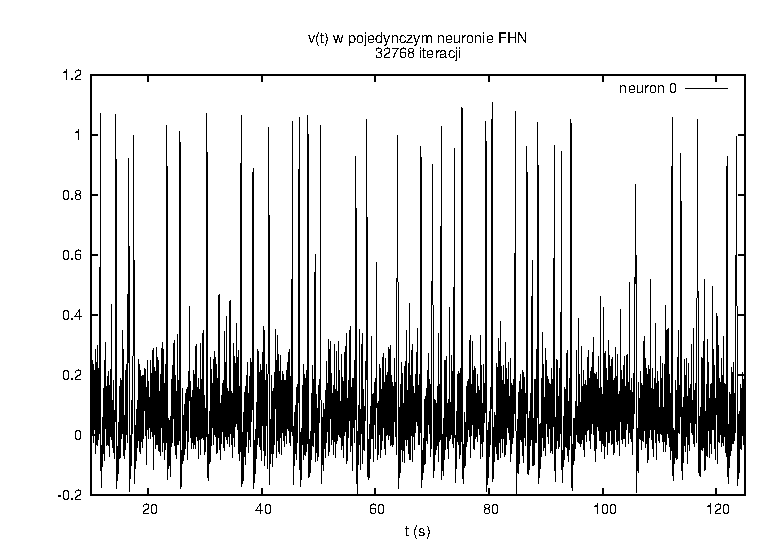
\includegraphics[width=140mm]{images/1neuron/1}} \\
        \resizebox{100mm}{!}{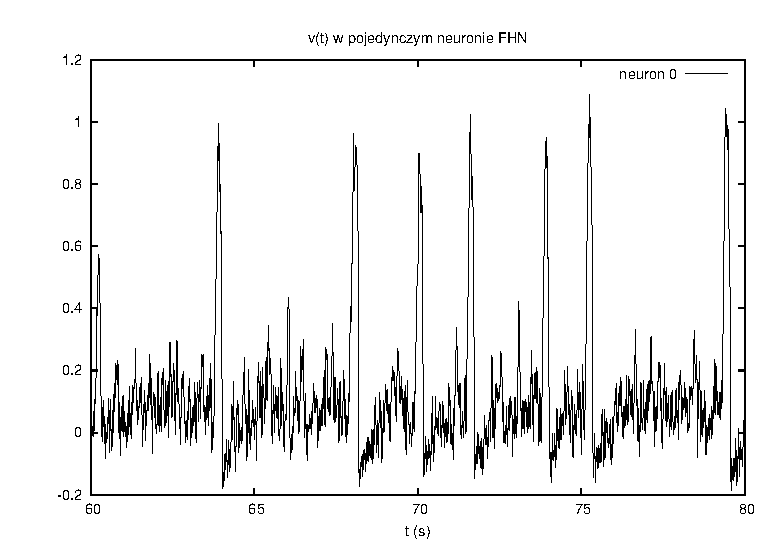
\includegraphics[width=140mm]{images/1neuron/2}} \\
      \end{tabular}
      \caption{Odtworzenie wyników Longtina (UZUPEŁNIĆ)}
      \label{sym1v}
    \end{center}
  \end{figure}

  Jest to przebieg zgodny z zaobserwowanym w pracy A. Longtin.

  \begin{figure}
    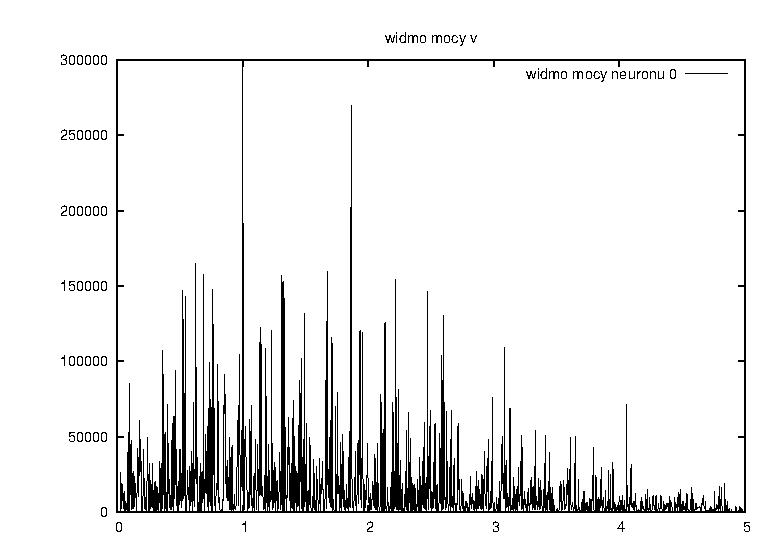
\includegraphics[width=140mm]{images/1neuron/3}
    \caption{FFT odtworzenie wyników longtina}
    \label{sym1fft}
  \end{figure}

  
  \subsection{Układy Neuronów Bez Opóźnienia}
  
  Następnym krokiem pracy było połączenie neuronów (początkowo dwóch) w ''sznur'', z sygnałem przekazywanym w jedną stronę, tzn. sygnał z neuronu i jest odbierany przez neuron i-1 (neuron o numerze 0 nie przekazuje swojego sygnału dalej). Neurony w układzie działały według równania zaproponowanego w rozdziale ~\ref{sec:przesuniecie_fazy}, bez opóźnienia (czyli $\tau_{n} = 0$)
  
  \begin{figure}
    \includegraphics[width=120mm]{images/pending}
    \caption{Układ kilku (?) neuronów bez opóźnienia. Widać wyraźny wzrost SNR zgodnie z ''kierunkiem'' przekazywania sygnału.}
    \label{fig:graphics:sim:x}
  \end{figure}

  Zaobserwowane przebiegi czasowe były zgodne ze spodziewanym analitycznie wynikiem: z każdym kolejnym neuronem w łańcuchu następował wzrost SNR (DO WARTOŚCI GRANICZNEJ) ze względu na wzrost prawdopodobieństwa wzbudzenia w przypadku wzbudzenia neuronu sąsiedniego.


  
  \subsection{Układy Neuronów Z Opóźnieniem}
  
  Do układu opisanego powyżej dodałem opóźnienie w przekazywaniu sygnałów, w sposób opisany w rozdziale ~\ref{sec:przesuniecie_fazy}

  \begin{figure}
    \includegraphics[width=120mm]{images/pending}
    \caption{Układ kilku (?) neuronów bez opóźnienia. Widać wyraźny wzrost SNR zgodnie z ''kierunkiem'' przekazywania sygnału.}
    \label{fig:graphics:sim:xx}
  \end{figure}
  
  
  \subsubsection{Macierz Dwóch Neuronów}

  Pierwszym krokiem w badaniu macierzy neuronów z opóźnieniem uczyniłem zbadanie macierzy dwuelementowej, celem znalezienia zależności pomiędzy podstawowymi parametrami symulacji.

  Przez c oznaczyłem opóźnienie transmisji, jako wielokrotność okresu sygnału periodycznego. Przesunięcie fazowe sygnału periodycznego p wynosiło pół okresu.
  Znaleziona zależność SNR (WYKRES) od c oraz D (skalowanie szumu) posiada bardzo wyraźną ''grań'' dla c=0.5, co potwierdza oczekiwania: maksymalizację SNR można osiągnąć poprzez kompensację przesunięcia fazowego (rozciągłości przestrzennej) identycznym (lub prawie identycznym) opóźnieniem w transmisji.

  \begin{figure}
    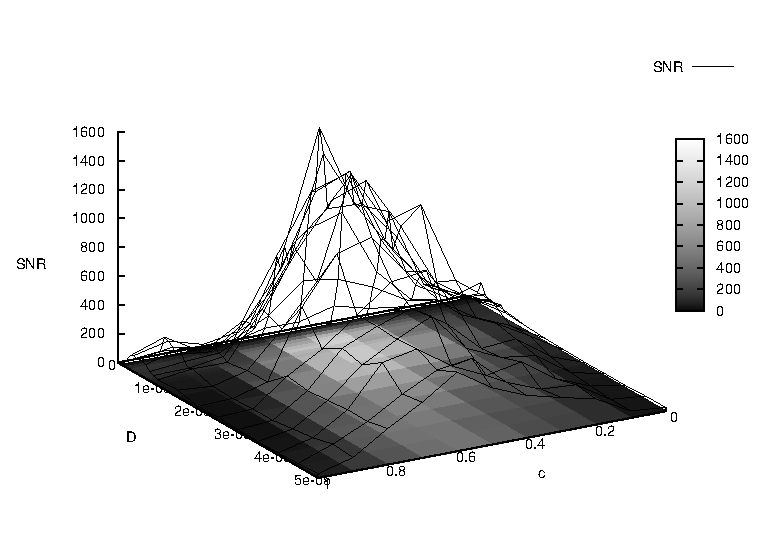
\includegraphics[width=140mm]{images/2neuron/3d}
    \caption{Dwa neurony, SNR w ''odbierającym'' w zależności od opóźnienia w transmisji c (jako wielokrotność T), dla przesunięcia fazowego równego 0.5T. Widać wyraźną ''grań'' kiedy c = p (= 0.5T)}
    \label{snr_c_d_3d}
  \end{figure}



  \newpage

    \section{Wnioski}
  
  Do uzupełnienia.
  \newpage
    
  
  \addcontentsline{toc}{section}{Literatura}
  \bibliographystyle{unsrtnat}
  \bibliography{bibliografia}
  
  
\end{document}
